% Full version only: batch shapes. Source: design/batching.md; measured
% sizes from spec/scripts/sizes.md and spec section 11 (REWRITE_h and
% DETACH_h are built, spec 7.9 and 7.10). The figure's coordinates are
% literal numbers from those sources.
\section{Batching}\label{sec:batching}

The path is most of a transition's cost, about $510\vB$ of a $1{,}020\vB$
exit at $D = 16$, so batching is the question of how many leaves can
share one. A transition has a fixed part (skeleton, state binding,
epilogue, control block; about $470\vB$) paid once per transaction, about
$32\vB$ per shared level paid once per path, and about 100 to $120\vB$
per leaf touched (its 116 bytes, signature, payout and hashing script),
which no shape removes (all three are read off the measured sizes).
Batching therefore helps only leaves under one aligned subtree, which
cohort grafts create and the sparse profile cannot.

\paragraph{The sweep.} \tr{EXIT}$_K$ chains single-leaf steps, each
with its full path, and saves only the skeleton ($665\vB$ for a second
exit). \tr{EVICT\_SUBTREE}$_h$ is the real batch: the witness carries the
path above an aligned subtree once and every position of the subtree,
the script folds the subtree in post order checking each lease and
evictor key, and folds the result and $\Emp_h$ up the shared path
($158\vB$ per leaf for 51 leaves). It is the operator's tool, and it
needs a lease on every leaf it sweeps.

\paragraph{The cohort rewrite, \tr{REWRITE}$_h$.} Running the sweep's
fold over two subtrees gives the general cohort transition. For each
position of an aligned subtree the witness carries an old and a new
element (a leaf or the empty string); the old root, folded from the old
elements, must fold with the shared path to $(r, S)$; the new root is
folded from the new elements; output~0 is
$(S - \sum\mathrm{old} + \sum\mathrm{new}, \TreeSpk(r', m))$, an increase
funded by other inputs. The owner of each changed leaf signs, except for
a leaf whose only change is a larger amount, and the operator signs once.
The rule that makes the rewrite a safe mass exit is the payout: a
position that goes from a leaf to $\Emp_0$ must be paid exactly its
amount, to its exit key, from the next unused output. An owner who signs
a transaction that empties its position is therefore paid by the
covenant, and the operator cannot remove a leaf without that owner's
signature and that payout; the owner multiproof of spec 13.4 is this
special case, not a separate script. In one transaction a cohort can
exit, join, resize, renew, rotate keys and pay between members with the
sum conserved, with only the members whose leaves change taking part:
the settlement step of an Ark round without a round, an expiry, or
unchanged members online.

Measured at $D = 16$, a rewrite in which every owner leaves costs 370,
198 and $159\vB$ per leaf for 4, 16 and 64 owners (\tr{REWRITE}$_2$,
\tr{REWRITE}$_4$, \tr{REWRITE}$_6$), the last within one vbyte of the
operator's sweep, and one in which all 64 owners rotate their keys costs
$145\vB$ per changed leaf, against $1{,}073\vB$ for an \tr{UPDATE} each.
\tr{REWRITE}$_6$ is 16{,}444 bytes of script. At $h = 6$ each position
costs 233 bytes of script and 234 of witness for its two elements, about
$117\vB$ whether or not it changes; an owner signature adds $16\vB$, and
an exit adds its 43-byte output and drops the new element, so an
unchanged position costs about $117\vB$, a changed one $133\vB$ and an
exiting one $147\vB$; the exit-consent form adds $16\vB$ per signed
position. The unchanged positions' bytes make it a tool for cohorts that
settle together. The Lean model covers it (\lean{rewrite\_sound}): the old and new subtrees
are published, so a cohort that joins this way is grounded by
construction and cannot be opaque, and a rewrite that empties the
subtree pays out exactly what it held
(\lean{rewrite\_exit\_conservation}).

\paragraph{Caching the path, \tr{DETACH}$_h$.} Script cannot read a
previous witness, so the upper levels of a cohort's path can only be
cached in an output of its own. \tr{DETACH}$_h$, signed by the operator,
proves an aligned subtree's node $(R_h, s_h)$ against $(r, S)$, leaves
$\Emp_h$ in output~0 for $S - s_h$, and creates output~1 as a depth-$h$
tree with root $R_h$, amount $s_h$ and a taptree $m_h$ fixed at creation;
members' paths truncated to the lower $h$ levels are their new proofs
(\lean{detach\_sound}, \lean{detach\_member\_payable}). At $D = 16$,
$h = 8$ it is 1{,}548 bytes of script and 497 of witness, about
$780\vB$, and every later exit from the detached tree costs the depth-8
figure, $765\vB$ instead of $1{,}020\vB$, so it pays for itself at the
fourth exit; a cohort of 256 that all leave alone saves about a quarter.
The larger effect is throughput: the cohort's exits form their own chain
of unconfirmed spends, so $\lat(N)$ applies to it separately, and the
operator can shard on demand when, say, channel leaves near their HTLC
deadlines. Vouchers bind $m$ and must be reissued under $m_h$; channel
leaves need nothing, as their $\mathsf{chan\_id}$ fixes $m$ at creation
and a detach leaves every leaf's bytes unchanged.

\begin{figure}[tbp]
\centering
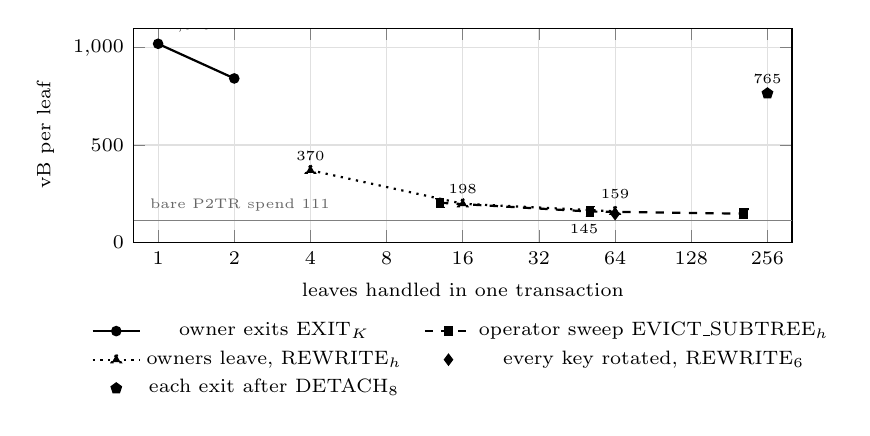
\begin{tikzpicture}
\begin{semilogxaxis}[
  width=0.82\linewidth, height=4.3cm, log basis x=2,
  xmin=0.8, xmax=320, ymin=0, ymax=1100,
  xtick={1,2,4,8,16,32,64,128,256}, xticklabels={1,2,4,8,16,32,64,128,256},
  xlabel={leaves handled in one transaction}, ylabel={vB per leaf},
  grid=major, grid style={black!12},
  legend style={at={(0.5,-0.32)}, anchor=north, legend columns=2, font=\scriptsize, draw=none, fill=none, /tikz/every even column/.append style={column sep=6pt}},
  tick label style={font=\scriptsize}, label style={font=\scriptsize}
]
\addplot[thick, mark=*, mark size=1.5pt] coordinates {(1,1020) (2,842)};
\addlegendentry{owner exits \tr{EXIT}$_K$}
\addplot[thick, dashed, mark=square*, mark size=1.5pt] coordinates {(13,203) (51,158) (206,147)};
\addlegendentry{operator sweep \tr{EVICT\_SUBTREE}$_h$}
\addplot[thick, dotted, mark=triangle*, mark size=1.8pt] coordinates {(4,370) (16,198) (64,159)};
\addlegendentry{owners leave, \tr{REWRITE}$_h$}
\addplot[only marks, mark=diamond*, mark size=2pt] coordinates {(64,145)};
\addlegendentry{every key rotated, \tr{REWRITE}$_6$}
\addplot[only marks, mark=pentagon*, mark size=2pt] coordinates {(256,765)};
\addlegendentry{each exit after \tr{DETACH}$_8$}
\addplot[black!50, thin, domain=0.8:320, samples=2] {111};
\node[font=\tiny, anchor=south west, black!60] at (axis cs:0.85,111) {bare P2TR spend 111};
\node[font=\tiny, anchor=south west] at (axis cs:1,1030) {1{,}020};
\node[font=\tiny, anchor=south] at (axis cs:4,370) {370};
\node[font=\tiny, anchor=south] at (axis cs:16,198) {198};
\node[font=\tiny, anchor=south] at (axis cs:64,175) {159};
\node[font=\tiny, anchor=north east] at (axis cs:60,140) {145};
\node[font=\tiny, anchor=south] at (axis cs:256,765) {765};
\end{semilogxaxis}
\end{tikzpicture}
\caption{Batch shapes at $D = 16$ on the model of \S\ref{sec:cost}, all measured: vbytes per leaf that leaves or changes against the leaves one transaction handles. The detach point is the cost of each later exit from a detached 256-leaf cohort, after a $780\vB$ detach.}
\label{fig:batching}
\end{figure}

Figure~\ref{fig:batching} places the shapes. Both new ones reuse the
sweep's post-order fold, and neither lowers the per-leaf floor: a leaf
that leaves costs its bytes, its signature and its output, about
$100\vB$, in every shape, and a leaf that stays in a rewritten subtree
costs about $117\vB$ because it is published twice.
